% ---------------------------------------------------------------------------------------------------------
\section{Why accuracy plateaus at about 0.57 on all patients}\label{sec:why}
More than 15 model families, 8 label-cleaning schemes, an external model trained on about 100,000 patients, and 3,313
class definitions all land at 0.55--0.57 four-class accuracy (0.63 with the ESC 2021 limits). The convergence points
to a limit in the \emph{information} carried by these printouts and labels, not in the modelling. The evidence:

\begin{enumerate}
  \item \textbf{EF precision vs band width.}
    \begin{itemize}
      \item The best header-free models estimate EF with $r\approx0.66$, residual SD about 13 points and MAE about 10.
      \item The Mild band (41 to 52/54) is about 12 points wide and the Moderate band 10.
      \item A simulation (true EF plus Gaussian error, cut at the class limits) gives an accuracy ceiling of 0.63 at
        SD 13. Reaching 0.73 needs SD 8, and 0.82 needs SD 5.
      \item The models reach 0.57--0.59, close to this ceiling.
    \end{itemize}
  \item \textbf{Errors sit at the class limits} (Figure~\ref{fig:boundary}).
    \begin{itemize}
      \item 51\,\% of ECGs have an echo EF within 6 points of a limit; their error rate is 62--68\,\%.
      \item ECGs at least 10 points from every limit are classified with 79--84\,\% accuracy.
      \item That clear-cut set contains no in-band Mild or Moderate ECG: those bands are too narrow.
    \end{itemize}
  \item \textbf{The ECG separates the extremes, not neighbouring grades.}
    \begin{itemize}
      \item Pairwise AUROC: Normal vs Severe 0.90 and Normal vs Moderate 0.88, but Normal vs Mild 0.75, Mild vs
        Moderate 0.63 and Moderate vs Severe 0.64.
      \item The best single Mild-vs-Moderate factor reaches 0.64.
      \item Mild differs from Normal mainly by conduction markers: QRS width, LBBB patterns.
    \end{itemize}
  \item \textbf{Label uncertainty.}
    \begin{itemize}
      \item EF comes from Teichholz M-mode reports.
      \item The echo is linked to the ECG by fuzzy name matching: only 44\,\% of ECGs have a clean link (exact name,
        echo within 30 days). 391 have a name-match score $<100$ and 192 an echo more than 30 days away.
      \item Repeat echoes of the same ECG differ by a median of 15.4 points (an upper bound).
      \item ECG--echo agreement is $r=0.75$ for clean links vs 0.42 for echoes more than 30 days away.
      \item Cleaning the labels changes all-ECG accuracy by only $-0.02$ to $+0.01$, because the remaining noise
        still exceeds the band width.
    \end{itemize}
  \item \textbf{Input format.}
    \begin{itemize}
      \item The PDFs give 2.5\,s per lead in four successive columns; only lead II covers 10 s.
      \item Foundation models were pre-trained on simultaneous 10-s digital ECGs.
      \item Reconstruction, multi-scale and per-column embeddings did not help. Digitisation quality was unrelated
        to error.
    \end{itemize}
  \item \textbf{Sample size.} 837 development ECGs, of which 185 are Mild. The learning curve gives $+1.4$ points per
    doubling, with no Mild trend.
\end{enumerate}

\begin{figure}[H]\centering
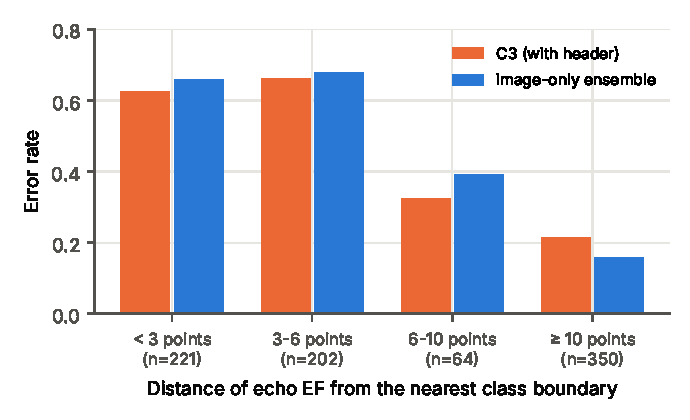
\includegraphics[width=0.62\linewidth]{figures/fig_error_vs_boundary.pdf}
\caption{Error rate by distance of the echo EF from the nearest class limit (all 837 ECGs, mean of 3 repeats).}\label{fig:boundary}
\end{figure}

\begin{figure}[H]\centering
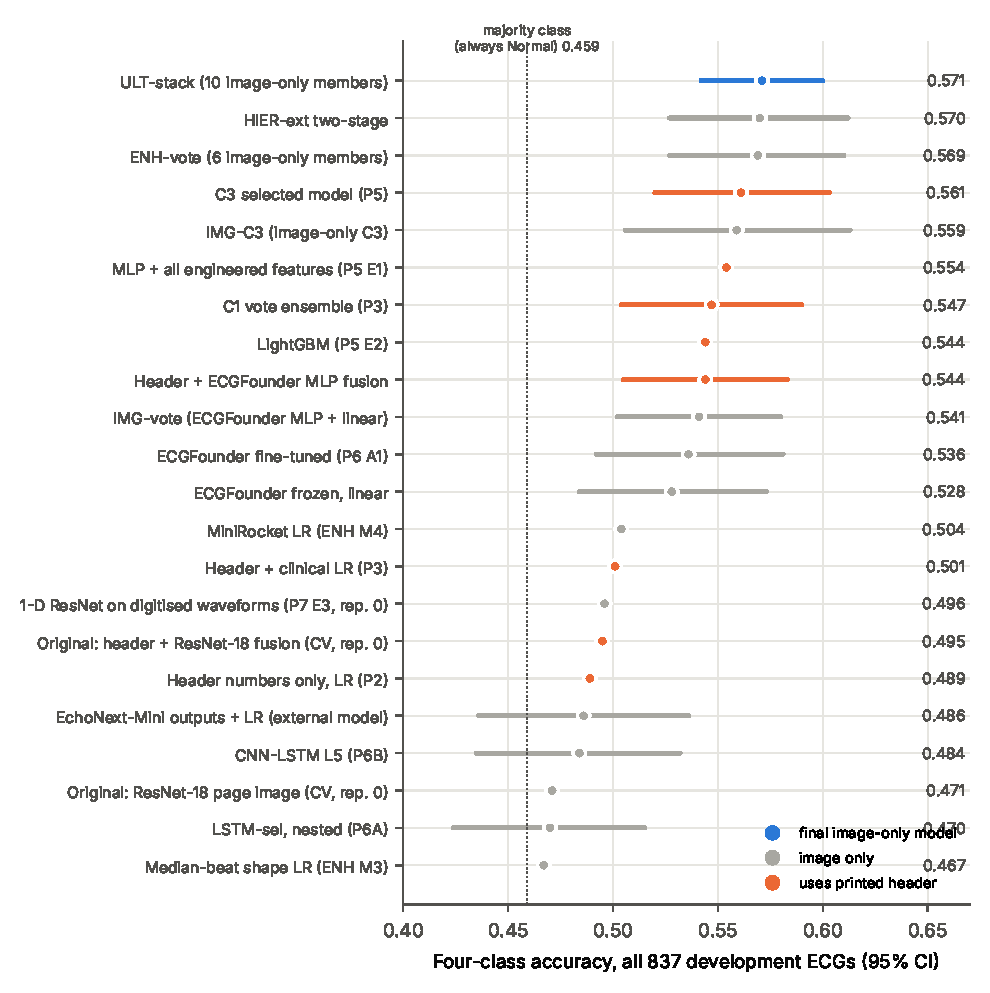
\includegraphics[width=0.92\linewidth]{figures/fig_model_landscape.pdf}
\caption{Four-class accuracy (all 837 development ECGs) of the main models across all phases. Image-only and
header-using models converge at 0.55--0.57.}\label{fig:landscape}
\end{figure}

% ---------------------------------------------------------------------------------------------------------
\section{Recommendations and ongoing work}\label{sec:future}
\begin{enumerate}
  \item \textbf{Verified ECG--echo linkage.} Link by MRN/UHID, with the echo within days and ideally in the same
    admission. A prioritised re-check worklist (197 high-priority ECGs, mostly Mild and Moderate) and a fill-in
    template are ready. A pipeline re-trains and re-scores the model as soon as verified data return; its self-test
    reproduces the current result exactly (\texttt{fixes.py}).
  \item \textbf{Biplane Simpson EF} instead of Teichholz, with repeat reads near the 41\,\% and 50--54\,\% limits.
  \item \textbf{Digital 10-s simultaneous ECGs} (XML/DICOM exports from the ECG machine) instead of PDF printouts.
  \item \textbf{More patients, enriched for Mild and Moderate.} At least 3,000 pairs, with at least 600 each of Mild
    and Moderate, preferably from a second centre.
  \item \textbf{Public-data pre-training (in progress, branch \texttt{research/public-ef}).}
    \begin{itemize}
      \item EchoNext (PhysioNet, credentialed) provides 100,000 ECGs with a numeric LVEF.
      \item Its ECGs are cut into the hospital printout layout, labelled with the same four-class rule, used for
        training, and then evaluated on the 837 development ECGs with the same folds.
      \item The data stay on the owner's laptop under the data-use agreement.
    \end{itemize}
  \item \textbf{A new prospective test set} scored once with the frozen test kit (\texttt{research/phase7-testkit}),
    because the locked set has now been used.
\end{enumerate}
